\chapter{Our approach}
\label{kap:approach}

\section{Inverse rendering}
As we explained in chapter \ref{kap:prior}, the two publications related to inverse rendering used improvements of SUNCG dataset. This dataset however, is subject to ongoing lawsuit \cite{suncg-lawsuit}, so authors of both papers could not made their datasets or trained models publicly available. At the time of writing this thesis, the lawsuit was still not resolved or settled, so we were not able to try and compare the trained models.
\newline
To solve this problem we decided to replicate paper by Sengupta et al. \cite{sengupta-inverse-rendering}, as it was easier to reproduce and thus would serve as better baseline moving forward. Our approach, however, was little different. As most of the materials in real world are not only made of diffuse component, but rather as combination of diffuse and specular part, we aimed to (on top of 3 properties estimated by Sengupta et al.) train neural network to also predict specular albedo, glossiness and view vector, i.e.\ to estimate all Phong parameters from one image. To do this, we extended IRN architecture by stacking more residual blocks for each added parameter.
\newline
As only diffuse albedo $\rho_d$, environment map and normals were estimated from IRN in the original paper, the only choice for BRDF was ideal diffuse BRDF defined as 
\begin{equation}
    \label{eq:diffuse-brdf}
    f_r = \frac{\rho_d}{\pi}
\end{equation}
When inspecting code for direct renderer written by Sengupta et al., we found out that the equation for computing direct illumination was as follows:
\begin{equation}
    f_{direct} = \frac{4\pi * \frac{\pi}{2}}{648} \sum_{i = 1}^{648} \frac{\rho_d}{\pi} * L(\omega_i) * (\omega_i \cdot N) 
    \label{eq:sengupta-direct}
\end{equation}
where 648 corresponds to 18x36 light directions (one for each pixel of the environment map predicted by IRN), $\rho_d$ stands for diffuse albedo (and thus the term $\frac{\rho_d}{\pi}$ for diffuse BRDF), $\omega_i$ for direction of incoming light vector, $L(\omega_i)$ for incoming illumination from direction $\omega_i$ (i.e.\ value of the corresponding pixel of the environment map) and $N$ for normal of the surface. Term $4\pi * \frac{\pi}{2} \; / \; 648$ corresponds to size of one pixel of environment map when mapped to sphere.
\newline
Equation \ref{eq:sengupta-direct} is incorrect, as pixels mapped closer to the poles of the sphere will occupy less sphere surface than those mapped closer to equator of the sphere. To account for this distortion, the contribution of incoming light from direction $\omega_i$ should be multiplied by the constant size of a pixel $ 4 \pi * \frac{\pi}{2} / 648$ times cosine of deviation of the direction from the equator, i.e. $\cos \theta_l$ for $\omega_i = (\theta_l, \phi_l)$ in spherical coordinates.
To summarize, fixed direct render function derived from equation \ref{eq:sengupta-direct} is then
\begin{equation}
    f_{direct} = \frac{4\pi * \frac{\pi}{2}}{648} \sum_{i = 1}^{648} \frac{\rho_d}{\pi} * L(\omega_i) * \cos \theta_l * (\omega_i \cdot N) 
    \label{eq:sengupta-direct-fix}
\end{equation}
\newline
As our modified IRN predicts all Phong parameters, we decided to use physically based Phong as our BRDF model. To recall, BRDF for physically based Phong is
\begin{equation}
    f^{Phong}_r = \frac{\rho_d}{\pi} + \frac{\rho_s(n + 2)\cos^n \theta_r}{2\pi}
\end{equation}
where $\rho_d$ and $\rho_s$ are diffuse and specular components respectively, $n$ stands for glossiness and $\cos^n \theta_r = (V \cdot R)^n$, $V$ representing view vector and $R$ corresponds to reflected vector, which is a light vector flipped according to normal and its calculation is specified in equation \ref{eq:reflected_vector}.
\begin{equation}
    R = 2(L \cdot N)N - L
    \label{eq:reflected_vector}
\end{equation}
In conclusion, our direct render function with physically based Phong BRDF is defined as
\begin{equation}
    f_{Phong} = \frac{4\pi * \frac{\pi}{2}}{648} \sum_{i = 1}^{648} \; (\frac{\rho_d}{\pi} + \frac{\rho_s(n + 2)\cos^n \theta_r}{2\pi}) \; * L_i(\omega_i) * \cos \theta_l * (\omega_i \cdot N)
    \label{eq:direct-phong}
\end{equation}
When implemented by matrix multiplication, our direct renderer function runs almost as fast as the original implementation of the direct renderer, even though our function deals with twice as many parameters. Comparison of results from original direct render function and our own implementation can be found in Appendix.
\section{Material Segmentation}
We tried to follow the transfer learning approach for material segmentation. As our primary goal is not to know precisely what is the class of the segmented material, our solution focused on material segmentation in the image without classification, which slightly simplifies the problem. When initialized, most architectures described in the previous chapter take number of classes as an argument, with this number describing how many feature maps should the model have in the output layer. To get a segmented image from neural network without post-processing (as we do not have the exact number of classes for materials in real world), we trained DeepLab model with 3 feature maps as output to mimic RGB image. To our surprise, the model was not able to learn underlying segmentation, even when trained from scratch, as shown in figure \ref{fig:deeplab-segmentation}.
\begin{figure}[H]
  \centering
  \begin{subfigure}{0.32\linewidth}
    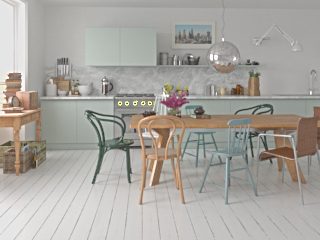
\includegraphics[width=\linewidth]{praca/images/AI43_001_Cam01.png}
    \caption{Original image}
  \end{subfigure}
  \begin{subfigure}{0.32\linewidth}
    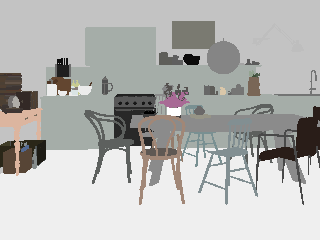
\includegraphics[width=\linewidth]{praca/images/AI43_001_Cam01.VRayMtlID.png}
    \caption{GT segmentation}
  \end{subfigure}
  \begin{subfigure}{0.32\linewidth}
    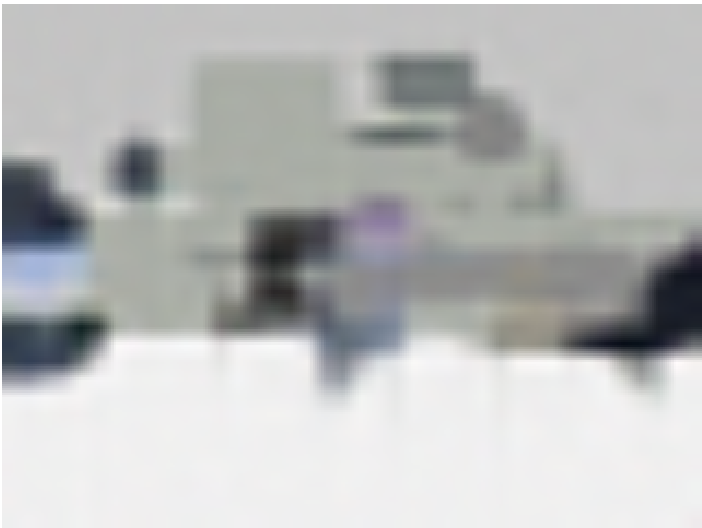
\includegraphics[width=\linewidth]{praca/images/DeepLab-segmentation.png}
    \caption{Predicted segmentation}
  \end{subfigure}
  \caption[Incorrect segmentation by DeepLab model]{Incorrect segmentation by DeepLab model}
  \label{fig:deeplab-segmentation}
\end{figure}
\noindent To solve this problem, we chose different architecture, in particular the one that we are using in IRN for estimating normals or albedo. This architecture had no problem to learn underlying segmentation, as presented in figure \ref{fig:proof-of-work-msn}. We named this network Material Segmentation Net, or MSN for short. Exact architecture of the model is described in section \ref{sec:msn-architecture}.
\begin{figure}[H]
  \centering
  \begin{subfigure}{0.32\linewidth}
    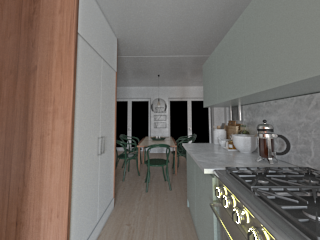
\includegraphics[width=\linewidth]{praca/images/AI45_007_Cam09.png}
    \caption{Original image}
  \end{subfigure}
  \begin{subfigure}{0.32\linewidth}
    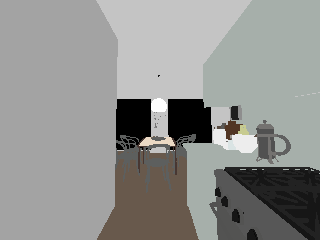
\includegraphics[width=\linewidth]{praca/images/AI45_007_Cam09.segmentation.png}
    \caption{GT segmentation}
  \end{subfigure}
  \begin{subfigure}{0.32\linewidth}
    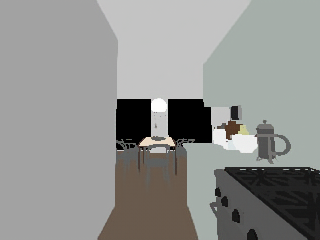
\includegraphics[width=\linewidth]{praca/images/AI45_007_Cam09.predicted_segmentation.png}
    \caption{Predicted segmentation}
  \end{subfigure}
  \caption[Proof of work - MSN]{Proof of work - MSN}
  \label{fig:proof-of-work-msn}
\end{figure}

